%% Corrects the page numbering, there is no need to change these
\cleardoublepage
\setcounter{page}{1}
\pagenumbering{arabic}

%% Leave first page empty \thispagestyle{empty}
\chapter{Introduction} 
The relationship between human beings and space has existed since the beginning of time. It has always been a source of mystery, something we want to understand. More than 4000 years ago, the Egyptians and the Babylonians were influenced by the movements of the sun and the planets and, based on those movements, developed calendars for their crops. Later, the ancient Greeks developed the concept of \emph{astronomy}, the science of the heavens. Other examples are philosophers such as Nicolaus Copernicus, Johannes Kepler, who explained the motion of the planets, and Galileo Galilei, who has been called the "father of modern observational astronomy" \cite{Singer}. In the 17th century, Sir Isaac Newton invented calculus, developed his law of gravitation and performed important experiments in optics.\\

The technological advancements of the 20th century, specially accelerated by the World War II, made physical exploration of space become possible. This exploration is mainly carried on by the use of satellites.\\

A \emph{satellite} is a natural or artificial object moving around a celestial body. This motion is described as an orbit, defined by the dominant force of gravity from the bigger body. In early 1945, the United States started the Vanguard Rocket development to launch a satellite. However, after several failed launches, it was de Soviet Union who took the advantage by launching the Sputnik-1 (Figure \ref{f1.1}) on October 4, 1957. Finally, on January 31, 1958 the United States managed to launch their first artificial satellite, the Explorer-1 (Figure \ref{f1.2}). During the Cold War, the space race between the two superpowers was a hard fight which made space technology advance quite rapidly.

\begin{figure}[H]
\centerline{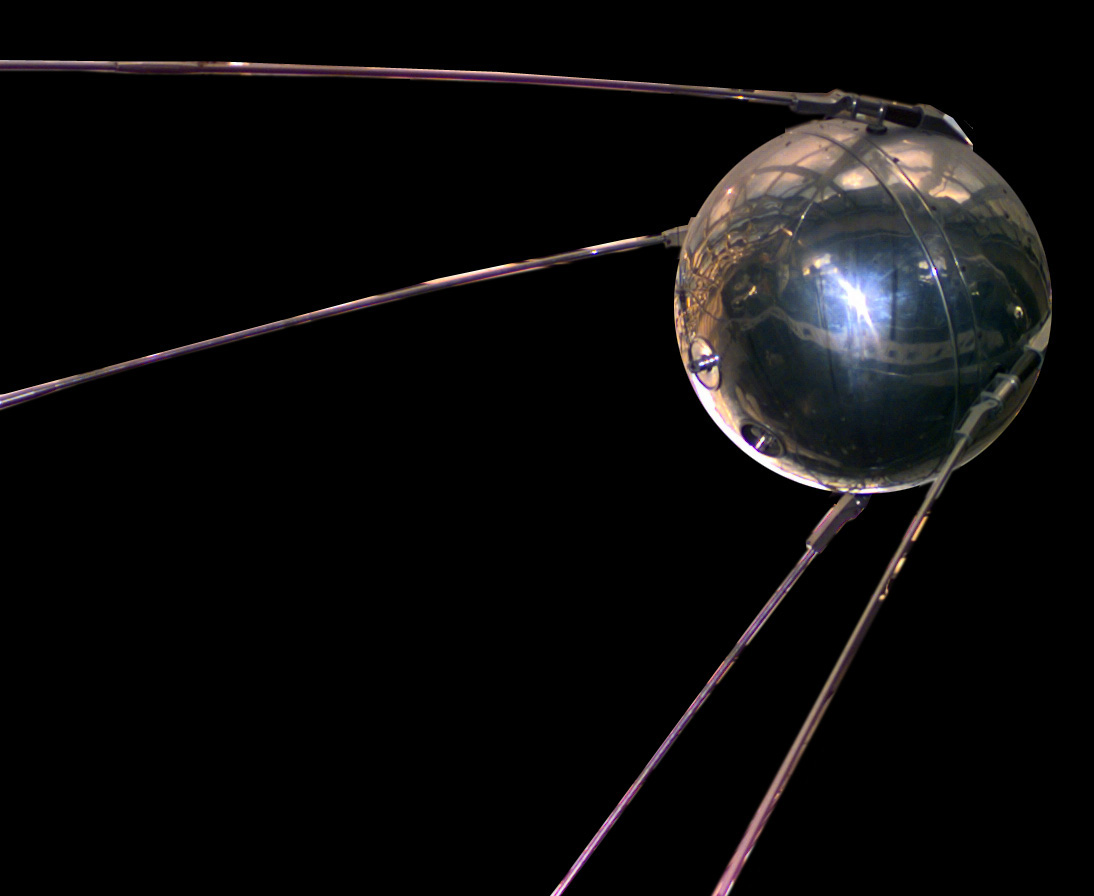
\includegraphics[width=0.7\textwidth]{images/sputnik.jpg}}
\caption{Sputnik 1, first artificial satellite launched by the Soviet Union in 1957  (National Aeronautics and Space Administration - Public Domain)}
\label{f1.1}
\end{figure}


\begin{figure}[H]
\centerline{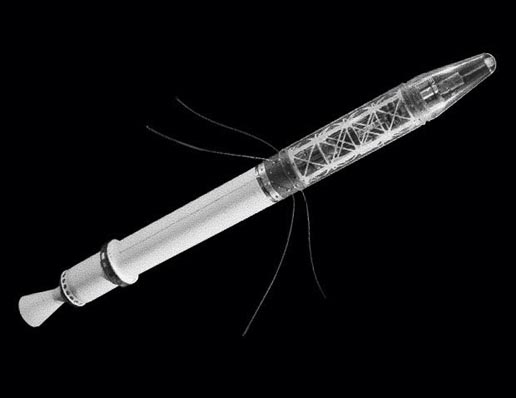
\includegraphics[width=0.7\textwidth]{images/explorer1.jpg}}
\caption{Explorer 1, first artificial satellite launched by the United States in 1958 (National Aeronautics and Space Administration - Public Domain)}
\label{f1.2}
\end{figure}
\pagebreak

As of October 1, 2011 there were 966 operating satellites in orbit. About two-thirds of these were owned by the United States, Russia and China \cite{SBFE}. Satellites can be divided into four main categories according to their usage:
\begin{itemize}
\item Communications satellites: used for television, radio, Internet and telephone services.
\item Navigation satellites: using radio time signals, these satellites allow mobile receivers on the ground to determine their exact position. They are also used to determine the location of satellites situated in lower orbits.
\item Exploration satellites: used to observe distant planets, galaxies and other outer space objects by using telescopes and other sensors.
\item Remote sensing satellites: Remote sensing satellites are used to gather information about the nature and condition of Earth. The sensors in this kind of satellites receive electromagnetic emissions in several spectral bands and can detect the object's composition and temperature, environmental conditions and so on. These satellites have sometimes also been used for military surveillance.

\end{itemize}

The constant evolution of technology and the growth of human needs have made the complexity and size of the satellites grow throughout the last decades. Satellite mass has grown from Sputnik's 84 kg and Explorer-1's 14k kg to Inmarsat-4's almost 6,000 kg in 2008 \cite{BARN}. The main consequence of this, amongst others, has been an increment in mission costs.\\

To counter this trend, the small satellite movement was created by the academic community and it has shown how mission costs can be cut dramatically to a point in which a university can build and launch their own satellite. (Figure \ref{f1.3}). The success of , it has become vigorous industry. Aalto University's student satellite Aalto-1 and Estonian student satellite ESTCube-1, projects with which this thesis is related, are nanosatellites, and the perfect example of this new movement.\\

\begin{figure}[H]
\centerline{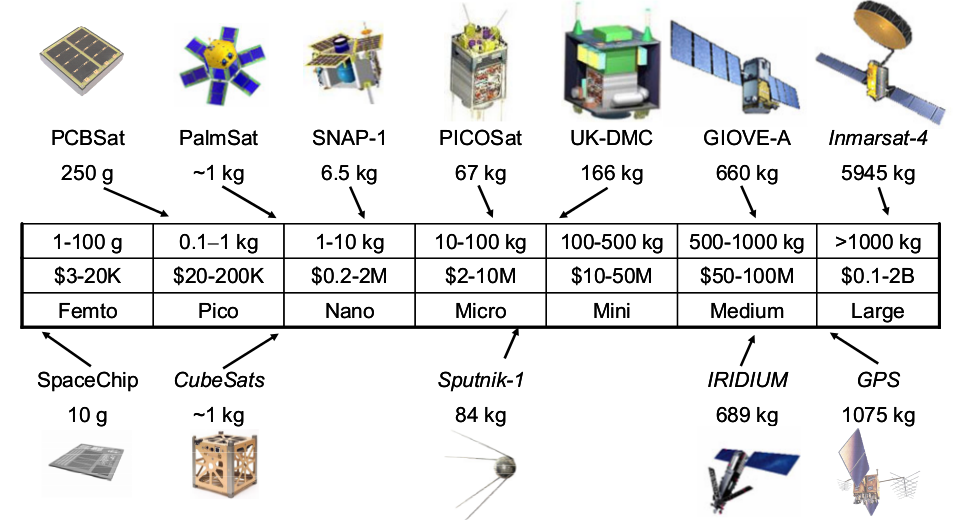
\includegraphics[width=0.7\textwidth]{images/satclass.png}}
\caption{Satellite Mass and Cost Classification \cite{BARN}}
\label{f1.3}
\end{figure}

\section{Background}\label{1.1}

This thesis is closely related to two different university based nanosatellite projects, Aalto-1 and ESTCube-1. These two projects are based on the most common standard use by universities: CubeSat\cite{CubeSat}, an open standard developed by the California Polytechnic State University and Stanford University.


\subsection{Aalto-1}

Led by Aalto University, Aalto-1 project aims to build a multi-payload remote sensing nanosatellite (Figure \ref{f1.4}). The size of the satellite is approximately 34 cm x 10 cm x 10 cm with a mass of less than 4 kg\cite{AALTO1a}. Aalto-1 also intents to be the first Finnish satellite.

\begin{figure}[H]
\centerline{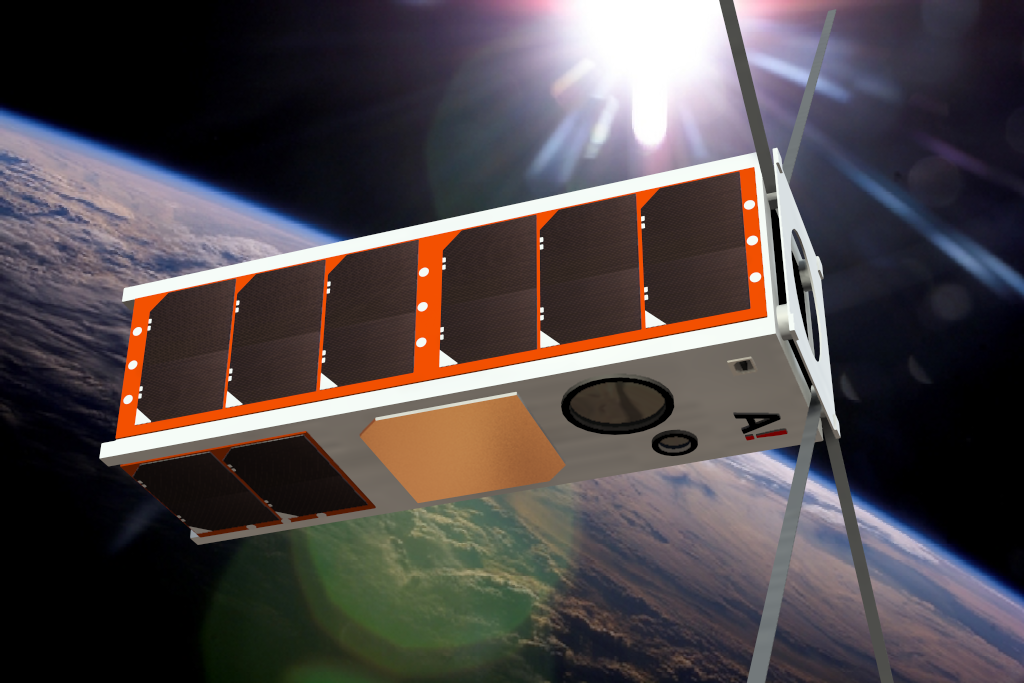
\includegraphics[width=0.7\textwidth]{images/aalto1.png}}
\caption{Aalto-1}
\label{f1.4}
\end{figure}


There are different institutions cooperating to make this possible. The main payload, the imaging spectrometer, has been designed and built by VTT Technical Research Centre of Finland. The Radiation Monitor (RADMON) has been designed by the Universities of Helsinki and Turku in cooperation with the Finnish Meteorological Institute (FMI). The Plasma Brake has been designed by a consortium including the FMI, the Department of Physics of the University of Helsinki, the Departments of Physics and Astronomy and Information Technology of the University of Turku, the Accelerator laboratory of the University of Jyväskylä, Aboa Space Resarch Oy, Oxford Instruments Oy and other Finnish companies. Meanwhile, Aalto University is responsible for designing and building the satellite platform and the day-to-day operation of the project. \cite{AALTO1b}\\ 

Aalto-1's mission is to demonstrate the technologies of the payloads in space environment and measure their performance. In addition, it is also an educational project. Students are the main workforce towards its success. Being the the first Finnish student satellite mission, is a good tool to improve Finnish space teaching and also allow students to be in touch with prominent partners, both domestic and international, in the space technology field.


\subsection{ESTCube-1}

ESTCube-1 is a single-unit CubeSat (Figure \ref{f1.5}). The size of the satellite is approximately 10 cm x 10 cm x 10 cm with a maximum mass of 1.33 kg. It has been build by students of the universities of Tartu and Tallinn, in Estonia, and it is the first Estonian satellite \cite{ESTCube}.
It was launched from the Guaiana Space Centre on May 7, 2013 as one of the three payloads of the Vega VV02 rocket \cite{Arianespace}.\\

\begin{figure}[H]
\centerline{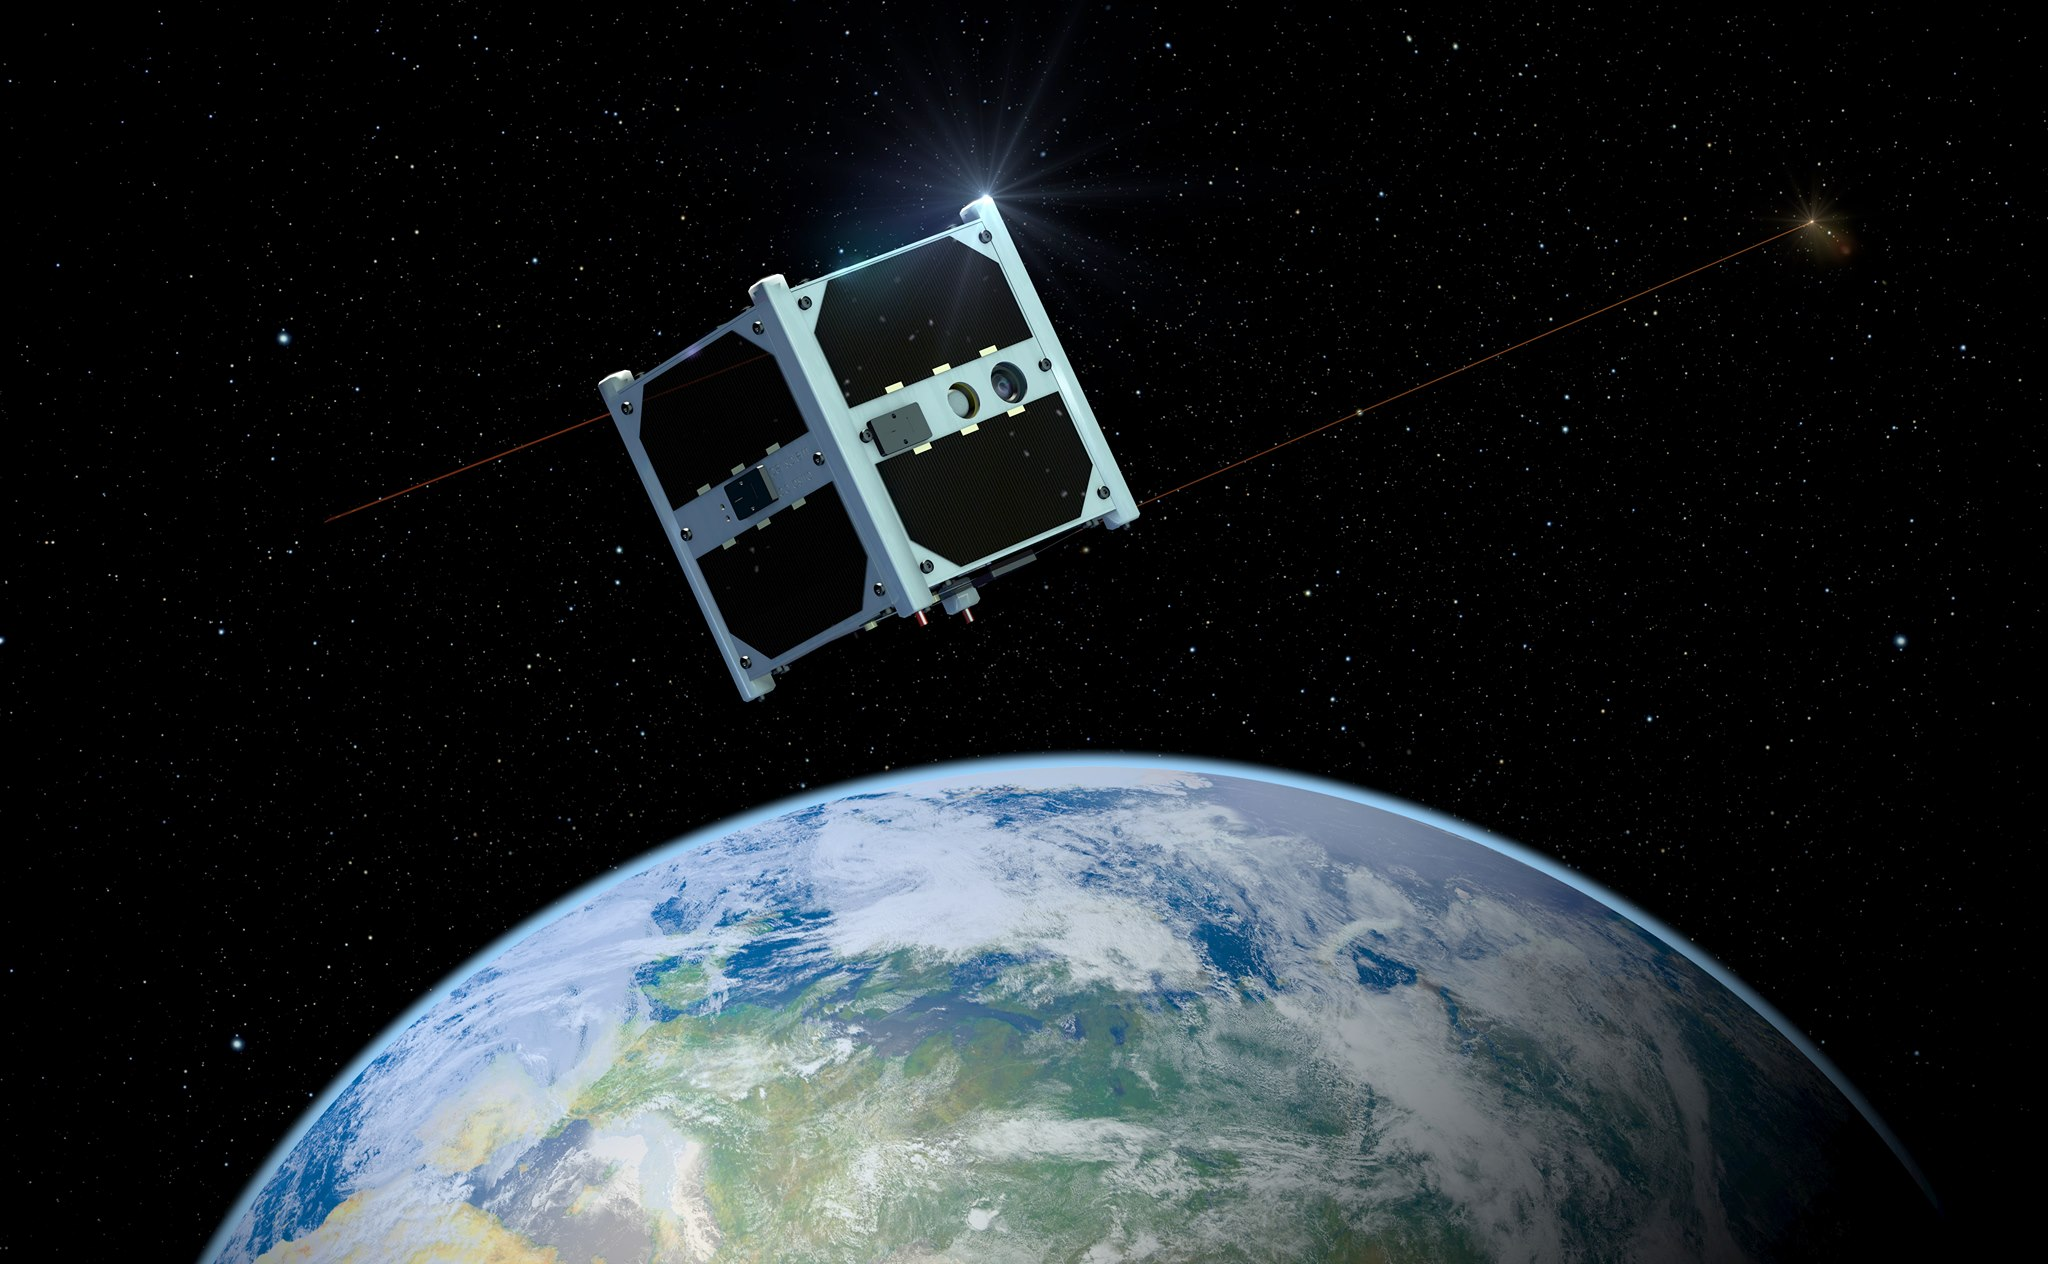
\includegraphics[width=0.7\textwidth]{images/ESTCube.jpg}}
\caption{ESTCube-1}
\label{f1.5}
\end{figure}

ESTCube-1's main goal is to observe and measure the E-sail effect for the first time. It has been placed into a polar low Earth orbit (LEO) and will deploy a single 10 m long and 9 mm wide tether \cite{ESTCube}. This has relation with Aalto-1's Plasma Brake, which will deploy a 100 m long tether. The require duration of ESTCube-1's mission is a few weeks and it can be extended to about a year.


\section{Problem statement}\label{1.2}

Any satellite mission is divided in two segments:
\begin{itemize}

	\item Space segment: the satellite.
	\item Ground segment this segment provides the means and resources to manage and control the data produced by the diverse instruments \cite{ESA}. 

\end{itemize}

The main part of the groud segment is the ground station, it is the first and final point of communication with the satellite, the place where the data is received and where the satellite is controlled from.


One of the main tasks of any mission is analysing the information received from its several sensors. However, the values generated by the sensors are not usually valid for scientific use as they are received, they are digital values which are not presented in any particular units and need to be calibrated.\\

The calibration process generates useful scientific values from those generated by the sensors. The equations to do so are provided by the vendors or calculated by experimentation before the launch. One of the main reasons for calibrating the values once they have been received by the ground station is saving downlink bandwidth. For example, a parameter C can be calculated based on the values of A and B, so it makes no sense to calculate it on board and waste downlink bandwidth to send C, when it can be done on ground.  In addition, the calibration equations might change over time, and it is much simpler to change something on the ground station software than on the satellite.\\


The received values also need to be checked to see if they are within the specified limits. This allows the scientists to discard invalid values or see how healthy the systems in the satellite are. These comparisons will generate several responses in the ground software, so again it only makes sense to do it on ground. 
\pagebreak

\section{Research objectives and scope}

The purpose of this thesis is to develop a calibration and a limit checking module for a ground control software which will solve the problems mentioned above.\\

Using ESTCube-1 project as a baseline, the author aims to develop such systems which are generic enough to be used by any number of satellite missions. The modules developed will be integrated into \emph{Hummingbird}, an open source platform for monitoring and control remote assets, which will be explained later in this work.\\ 
The following items support this purpose:
\begin{itemize}
	\item Research about satellite orbits and how they affect satellite-Earth communications.
	\item Research about what types data are exchanged between satellites and ground stations.
	\item See what are the different parts of a ground station, including hardware and software pieces.
	\item Present the most common protocols used for amateur satellite communications. 
\end{itemize}

\section{Motivations}

When the moment came to choose a software solution for Aalto-1's ground station, the approach was to develop something ad-hoc for the mission. There was no available software which was good enough for the mission's requirements unless it was oriented for big processional satellites. However, due to the cooperation with the University of Tartu, \emph{Hummingbird} came into play as a real strong option. It is an open source project which, in addition to controlling the ground station and satellite, also aims to create a network of ground stations around the world. 

The development of this product will not only benefit both, Aalto University and the University of Tartu. Being open source, any mission can use a ready-to-use, fully tested software as a baseline for their ground control systems, which will help small satellite missions shorten their development time frames. 

\pagebreak
\section{Outline of the thesis}
This thesis is structured as follows: the second chapter gives a general overview about satellite communications, how orbits affect these, what data is transmitted and what are the different protocols, hardware and software components to do so. The third chapter explains briefly what Hummingbird is and what is behind it. The fourth chapter goes through the requirements set for the software project whereas the fifth one focuses on the design and implementation. Chapter six comprises a short user manual. Chapter six summarizes the conclusions of this thesis. Finally, chapter seven explains what are the next steps in the project.

\newpage
